\documentclass[preview]{standalone}
\usepackage{pgfplots}
\begin{document}
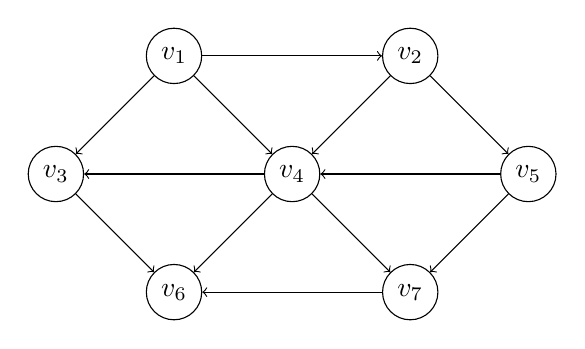
\begin{tikzpicture}[node distance={15mm}, main/.style = {draw, circle}]
\tikzstyle{vertex}=[circle,draw=black,fill=white,minimum size=20pt, inner sep=0pt]
\node[vertex] (A) at (0, 0) {\(v_1\)};
\node[vertex] (B) at (3, 0) {\(v_2\)};
\node[vertex] (C) at (-1.5, -1.5) {\(v_3\)};
\node[vertex] (D) at (1.5, -1.5) {\(v_4\)};
\node[vertex] (E) at (4.5, -1.5) {\(v_5\)};
\node[vertex] (F) at (0, -3) {\(v_6\)};
\node[vertex] (G) at (3, -3) {\(v_7\)};
\path[->]
(A) edge (B)
(A) edge (C)
(A) edge (D)
(B) edge (D)
(B) edge (E)
(C) edge (F)
(D) edge (C)
(D) edge (F)
(D) edge (G)
(E) edge (D)
(E) edge (G)
(G) edge (F)
;
% (B) -- node[above]{8} (C)
% (C) -- node[above]{7} (D)
% (D) -- node[anchor=south west]{9} (E)
% (E) -- node[anchor=north west]{10} (F)
% (A) -- node[anchor=north east]{8} (H)
% (B) -- node[left]{11} (H)
% (D) -- node[right]{14} (F)
% (H) -- node[anchor=south east]{7} (I)
% (I) -- node[anchor=south west]{6} (G)
% ;
% \draw[ultra thick,red]
% (G) -- node[below]{1} (H)
% (I) -- node[anchor=south east]{2} (C)
% (F) -- node[below]{2} (G)
% (C) -- node[anchor=south west]{4} (F)
% (A) -- node[anchor=south east]{4} (B)
% ;
\end{tikzpicture}
\end{document}